\documentclass[12pt]{article}

\usepackage{sbc-template}

\usepackage{graphicx,url}

\usepackage[brazil]{babel}   
%\usepackage[latin1]{inputenc}  
\usepackage[utf8]{inputenc}  
% UTF-8 encoding is recommended by ShareLaTex

     
\sloppy

\title{Pesquisa sobre as tecnologias Skype Translator e Algoritmo Procedural}

\author{Diego F. Sousa Lima\inst{1},Bruno L. Alcântara\inst{1} }


\address{Curso Bacharelado em Sistemas de Informação -- Universidade Federal do Piauí
	(UFPI)\\
	Junco, Picos -- PI, 64600-000 -- Brazil
	\email{\{diegofernando5672,brunolopes.ips\}@gmail.com}
}
\begin{document} 

\maketitle

\begin{abstract}
  Este meta-artigo descreve uma pesquisa feita acerca das novas tecnologias do Skype (em especial a Skype Translator) e Algoritmo Procedural aplicado ao jogo No Man’s Sky.
\end{abstract}
     
\begin{resumo} 
 This meta-article describes a research done on the new technologies of Skype (in particular a Skype Translator) and Procedural Algorithm applied to the game No Man's Sky.
\end{resumo}


\section{Skype Translator}

\subsection{Histórico e definição}

O projeto Skype Translator visa permitir conversas de domínio aberto entre usuários em diferentes partes do mundo em línguas diferentes. Além de permitir maior poder de comunicabilidade entre as partes, essa tecnologia também permite a comunicação Skype com outra classe de usuários: aqueles que têm surdez ou dificuldades auditivas.

De acordo com Lewis, pesquisador da Microsoft, Skype Translator surgiu baseado no filme Star Trek de 1966. No caso, o filme nos introduziu uma noção de “tradutor universal”, pois, há um dispositivo no qual o Capitão Kirk e sua tripulação se comunicam com espécies exóticas, como o Gorn, que não falavam sua língua.

Embora a comunicação sem falhas usando tecnologia de fala e tradução esteja além do estado atual da arte, grandes melhorias nestas tecnologias ao longo da última década nos trouxeram muitos passos mais próximos. O  Skype Translator reúne o atual estado da arte nessas tecnologias e fornece um serviço de tradução de fala em um serviço de Voz sobre Internet (VoIP), ou seja, Skype.
Com o Skype Translator, um usuário do Skype que fala, por exemplo, inglês, pode ligar para um colega ou amigo que fala, digamos, espanhol, e ser capaz de manter uma conversa bilíngue mediada pelo tradutor.

\subsection{Funcionamento} \label{sec:firstpage}

O Skype Translator é um pipeline do estilo speech-to-speech (S2S). Este consiste em três elementos principais:

\begin{itemize}
	\item Automated Speech Recognition (ASR) – Reconhecimento automatizado de fala;
	\item Machine Translation (MT) engine  – Mecanismo de tradução automática;
	\item Text-to-Speesch (TTS) – Texto para conversa.
\end{itemize}

Primeiramente, o ASR converte um sinal de áudio de entrada em texto, essencialmente “transcrevendo” as palavra faladas em palavras escritas. Cada linguagem tem um próprio mecanismo construído personalizado, e geralmente requer centenas de milhares de horas de conteúdo transcritos por humanos para o treinamento do ASR.

A MT é baseada em métodos estatísticos, assim como o Microsoft Translator e o Google Translator, e aprende com dados paralelos um mapeamento probabilístico entre palavras e frases em um idioma para traduções.

Por último, o TTS mapeia o texto em uma linguagem para uma forma falada, e geralmente é treinado cuidadosamente gravado ou transcrições de um falante nativo.

Com essas três tecnologias, aparentemente que o que deve ser feito é apenas conectá-las umas as outras para construir um pipeline S2S, porém, não é tão simples assim. O problema se tem início com os usuários, pois a maioria dos não falam fluentemente ou não conseguem falar uma palavra corretamente. Isso pode comprometer drasticamente o conteúdo final da mensagem.

\begin{figure}[ht]
	\centering
	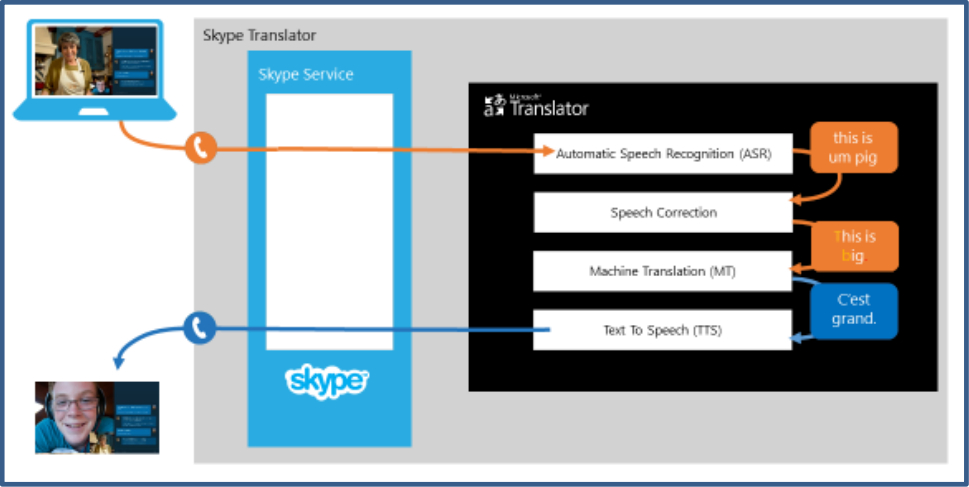
\includegraphics[width=.5\textwidth]{imagem1pdsi.jpg}
	\caption{Exemplo de conversa.}
	\label{fig:imagem1pdsi}
\end{figure}

\subsection{A técnica de Crowdsourcing}

Existe uma tendência crescente entre algumas empresas de software de internet para envolver os usuários no processo de tradução, convidando ou capacitando-os a moldar a forma como o produto final lê em suas línguas nativas. Isso é chamado de crowdsourcing de tradução.

O caso do Skype é tratado com tecnologia fechada. Neste modelo, a empresa limita a adesão da multidão e age para pré-selecionar os usuários-tradutores que podem participar do projeto de tradução. Assim, a adesão está sujeita a cumprir determinados requisitos. Isso significa que a comunidade é mais exclusiva, e pertencer à comunidade também pode colocar certas obrigações na multidão, por exemplo, acordos de confidencialidade e prazos de tradução. Essas obrigações, por definição, não recaem sobre os participantes de uma comunidade aberta.

Modelos comunitários fechados estão se tornando uma tendência predominante no crowdsourcing de tradução na indústria de software (Ray e Lommel 2009, 59). O Skype realmente implementa dois tipos diferentes de modelos de crowdsourcing - um para seus chamados idiomas oficiais (multidão fechada) e outro que permite a qualquer pessoa traduzir o Skype para qualquer outra língua (multidão aberta). Este artigo analisa o modelo fechado. Além de oferecer traduções, o Skype usa a ajuda da comunidade para outros aspectos da localização. Por exemplo, os tradutores ajudam a verificar se as normas específicas da localidade são levadas em conta; As listas são exibidas na ordem alfabética correta; E as datas são exibidas corretamente etc. Em outras palavras, eles não apenas olham para as cadeias traduzíveis, mas para a imagem de localização maior.

\section{Algoritmo Procedural}

\subsection{No Man's Sky - O jogo}

No Cenário atual, os jogos eletrônicos já são um tipo de entretenimento já consolidado na sociedade. Podemos encontrar jogos dos mais diversificados gêneros, como esportes, ação, estratégia, jogos de tabuleiro exploração, etc. Dentre os variados gêneros existentes, há um gênero de jogo conhecido como mundo aberto (do inglês Open World) que permite o jogador explorar livremente o mundo virtual do jogo. Por conta disso, surgiram à vocação de produzir jogos com extenso uso de elementos de geração automática principalmente como mapas, cenários, itens, etc. Tal técnica, denominada Geração Procedural de Conteúdo (PCG), ganhou notável reconhecimento nos últimos anos, devido aos efeitos obtidos com seu uso. Pensando nisso, a Hello Games desenvolveu um jogo utilizando essa tecnologia chamada: No Man’s Sky.

No Man’s Sky é um jogo de exploração espacial, coleta de recursos e troca. Todo o universo do jogo é criado de forma procedural. Todos os aspectos gráficos como animais, terrenos, vegetação e alguns aspectos mecânicos como planetas e galáxias são criados por algoritmos procedurais. Ao todo, o jogo consegue gerar 18.446.744.073.709.551.616 planetas distintos. O jogo utiliza sistemas de Lindenmeyer, sistemas de gramática formal e geradores de números pseudoaleatórios para criar um valor seed, após ser processado pelo motor do jogo, sempre gera o mesmo resultado, permitindo que os diversos jogadores visitem o mesmo planeta diversas vezes, sem que haja alterações físicas nele. Esse resultado pode ser qualquer conteúdo dentro do espaço virtual.



\subsection{Geração Procedural de Conteúdo}\label{sec:figs}


Um aspecto frequentemente encontrado em alguns jogos de mundo aberto é a geração de conteúdo procedural, que corresponde à criação programática de conteúdo do jogo, através de processos estocásticos ou pseudoaleatórios, gerando uma gama de resultados imprevisíveis no espaço do jogo, de maneira que sempre afeta sua jogabilidade em algum sentido. Nesses casos, é comum a aleatoriedade ser controlada a partir de alguns parâmetros e ser possível gerar uma grande abundância de possíveis conteúdos considerados “válidos”. Exemplos de geração procedural de conteúdo em jogos incluem construção de labirintos, personagens, mapas, planetas inteiros ou até histórias em tempos de execução. É possível descrever o comportamento de sistemas de PCG, quando em conjunto com o trabalho de um designer em quatro metáforas:

\begin{itemize}
	\item Ferramenta: um sistema pode ser compreendido como um mecanismo ou um dispositivo manipulado com o intuito de alcançar um objetivo no game design, que aprimora as habilidades de um designer;
	\item Materiais: são “substâncias” dinâmicas, reconfiguráveis e geradas “procedural mente” que podem ser manipuladas e moldadas pelo game designer para alcançar um objetivo;	
	\item Designers: são algoritmos ou sistemas PCG que são responsáveis por resolver problemas de game design e executar tarefas de design com pouca ou nenhuma intervenção de um designer humano;
	\item Expert: Um algoritmo ou sistema PCG Expert pode ser dividido em Player Expert e Domain Expert. Ambos analisam e interpretam os estados do jogo e, normalmente, são empregados em serious games. Enquanto o Player Expert é responsável pela informação referente às ações do jogador, o Domain Expert manipula informações dos outros aspectos do jogo, como mapas e terrenos. Geralmente, Experts não requerem interação com designers.
\end{itemize}

\subsection{Motivo para se utilizar Geração Procedural de Conteúdo}

A quantidade de funcionários e custo dos jogos modernos é cada vez maior e o algoritmo procedural serve como alternativa, já que funcionários humanos são caros e comparativamente lentos. Esse alto custo torna os projetos menos lucrativos e mina a capacidade da indústria de criar jogos inovadores e diversos, por medo de prejuízo. Se um estúdio desenvolvedor consegue cortar gastos de produção, de forma mais rápida e barata e ainda mantendo a qualidade, ele tem uma clara vantagem competitiva. Isso não significa que o designer humano deve, ou virá a ser substituído por algoritmos procedurais. As técnicas de geração de conteúdo podem aumentar a capacidade criativa de designers humanos, sendo ferramentas na construção de conteúdo único e/ou inovador.

\subsection{Paradigmas de Geração Procedural de Conteúdo}

As características dos conceitos de Geração Procedural de Conteúdo resultam em diversas formas de elaboração e pode fazer com que desenvolvedores tenham dúvidas sobre qual a melhor abordagem para a resolução de problemas. É necessário, então, definir os paradigmas que regem tais implementações descrevem diversos paradigmas em e o conteúdo é revisitado posteriormente. 

\subsubsection{Online versus offline}

A geração do conteúdo por um algoritmo procedural pode ser feita em dois momentos. Se o conteúdo é gerado enquanto o jogador utiliza o ambiente virtual, gerando infinitas variações ou permitindo que o jogo se adapte às ações do jogador de forma dinâmica, o algoritmo PCG é chamado de Online. Do contrário, se o algoritmo faz sua função antes do jogo começar ou até mesmo durante o processo de desenvolvimento do software, ele é chamado de Offline. 

\subsubsection{Necessário versus Opcional }

Um algoritmo pode ser utilizado para gerar conteúdo que é necessário para que uma fase ou o próprio jogo seja completo. A delegação da geração de conteúdo essencial para um jogo como necessário. Todo e qualquer resultado vindo desse algoritmo deve ser sempre correto. O PCG pode, porém, gerar aspectos secundários de um jogo, como algumas texturas, uma casa ou vilarejo que pode ser ignorado pelo jogador etc. Se esse conteúdo pode ser substituído posteriormente ou excluído sem perda da lógica do jogo, o PCG é chamado de opcional.

\subsubsection{Genérico versus adaptável}

Se o conteúdo do jogo, ao ser gerado, não leva em consideração o comportamento do jogador, pode-se dizer que foi proveniente de um PCG genérico. Do contrário, ele é adaptável. É importante ressaltar que a adaptabilidade de um sistema PCG pode ter implicações grandes no campo de interação humano-computador (IHC). 

\subsubsection{Seeds aleatórios versus vetor de parâmetros}

Um seed é uma sequência de números semi aleatórios usados como valor de entrada ou saída de um algoritmo qualquer (podendo ou não ser um algoritmo PCG). É importante saber até que ponto o algoritmo gerador pode ser parametrizado. Quase todos os algoritmos PCG geram algum tipo de conteúdo “expandido”, baseado em um valor de input. A distinção entre os paradigmas ocorre na forma que o algoritmo recebe tal entrada, seja ele um valor seed semi aleatório ou um vetor multidimensional altamente parametrizado.

\subsubsection{Geração automática versus autoria mista}

O conceito de geração automática é proveniente da delegação da criação do conteúdo somente para o algoritmo PCG, tendo nenhuma ou pouquíssima interação humana. Já a autoria mista é a junção do processo de criação PCG com a intervenção significativa de designers humanos. 

\section{Conclusão}

No Skype Translator, é perceptível a contribuição para o âmbito social como também a inclusão. É uma tecnologia que está em plena fase de amadurecimento, basta observar um dos seus maiores problemas que é mudar totalmente o sentido de uma frase quando o emissor não omite o som das palavras com certa exatidão. Talvez isso seja um grande obstáculo.

Já no Algoritmo Procedural, a retomada de interesse pelos PCG acarreta a necessidade de formas inovadoras de criação e elaboração de diversas técnicas. É possível que no futuro tenhamos jogos criados inteiramente por máquinas e algoritmos. As possibilidades e o potencial dos algoritmos procedural são quase imensuráveis.
A abordagem desse mecanismo poderoso no desenvolvimento de jogos podendo até serem aliado a diversas áreas do conhecimento, como a matemática e até a biologia, Fractais, linguagens formais, educação, etc. Existem diversas outras técnicas de geração de conteúdo. A gama de aplicações das técnicas expostas é vasta.   



\bibliographystyle{sbc}
\bibliography{sbc-template}

\end{document}
